\documentclass{solutionclass} % I wrote the design using a4paper, 11pt, twoside, but feel free to change in solutionclass.cls file (line 4)
\usepackage{subcaption}
\pagestyle{plain}

\lstdefinestyle{mystyle}{
	backgroundcolor=\color{backcolour},
	commentstyle=\color{codegreen},
	keywordstyle=\color{magenta},
	numberstyle=\tiny\color{codegray},
	stringstyle=\color{codepurple},
	basicstyle=\ttfamily\normalsize,
	breakatwhitespace=false,
	breaklines=true,
	captionpos=b,
	keepspaces=true,
	numbers=left,
	numbersep=5pt,
	showspaces=false,
	showstringspaces=false,
	showtabs=false,
	tabsize=2
}

\lstset{ %
	language=Python,       % the language of the code
	basicstyle=\footnotesize,       % the size of the fonts that are used for the code
	numbers=left,                   % where to put the line-numbers
	numberstyle=\tiny\color{gray},  % the style that is used for the line-numbers
	stepnumber=1,                   % the step between two line-numbers. If it's 1, each line
	% will be numbered
	numbersep=5pt,                  % how far the line-numbers are from the code
	backgroundcolor=\color{white},  % choose the background color. You must add \usepackage{color}
	showspaces=false,               % show spaces adding particular underscores
	showstringspaces=false,         % underline spaces within strings
	showtabs=false,                 % show tabs within strings adding particular underscores
	frame=single,                   % adds a frame around the code
	rulecolor=\color{black},        % if not set, the frame-color may be changed on line-breaks within not-black text (e.g. commens (green here))
	tabsize=4,                      % sets default tabsize to 2 spaces
	breaklines=true,                % sets automatic line breaking
	breakatwhitespace=false,        % sets if automatic breaks should only happen at whitespace
	% also try caption instead of title
	keywordstyle=\color{blue},
    emph=[1]{for,if, end,break},emphstyle=[1]\color{red},         % keyword style
	commentstyle=\color{dkgreen},       % comment style
	stringstyle=\color{mauve},         % string literal style
	escapeinside={\%*}{*)},            % if you want to add a comment within your code
	morekeywords={*,...}               % if you want to add more keywords to the set
}

\hypersetup{
	colorlinks   = true, %Colours links instead of ugly boxes
	urlcolor     = blue, %Colour for external hyperlinks
	linkcolor    = blue, %Colour of internal links
	citecolor   = red %Colour of citations
}

\definecolor{codegreen}{rgb}{0,0.6,0}
\definecolor{codegray}{rgb}{0.5,0.5,0.5}
\definecolor{codepurple}{rgb}{0.58,0,0.82}
\definecolor{backcolour}{rgb}{0.95,0.95,0.92}
\definecolor{mGreen}{rgb}{0,0.6,0}
\definecolor{mGray}{rgb}{0.5,0.5,0.5}
\definecolor{mPurple}{rgb}{0.58,0,0.82}
\definecolor{backgroundColour}{rgb}{0.95,0.95,0.92}

\NewDocumentCommand{\codeword}{v}{
	\texttt{\textcolor{blue}{#1}}
}

\definecolor{dkgreen}{rgb}{0,0.6,0}
\definecolor{gray}{rgb}{0.5,0.5,0.5}
\definecolor{mauve}{rgb}{0.58,0,0.82}

\def\m#1{\boldsymbol{#1}}
\def\co#1{\texttt{#1}}


\begin{document}

\pretitle
{HomeWork 4} % ⟸ Write your main Title here
{Ilia Hashemi Rad}
{99102456}
{AmirMohammad Fakhimi}
{99170531}
{AmirMahdi Namjoo}
{402211467}

% Change your homework number here
\def\homeworkNumber{2}

\makeatletter
    \startcontents[sections]
    \phantomsection
\makeatother
    \def\Solu{Explanations}

\section{Introduction}

\begin{solution}
    In this project, we have implemented a Transformer model that tries to identify and neutralize gender bias in texts. To achieve this, we first gathered a dataset consisting of Persian tweets with gender bias and some ChatGPT responses with gender bias. We then investigated them manually, removed identical data automatically, and too similar data manually to reach a general and diverse data of 1455 size. We then used LLMs to neutralize gender bias in these texts. We then fine-tuned an LLM on these data and evaluated the results in each part.


We should also mention that we used "Identifying and Neutralizing Gender Bias from Text" from Stanford University to get some ideas for the implementation. Notably, the article is based on the English language, and we did not have access to its dataset or code.

It is noteworthy that a dataset called "EXIST" exists for gender bias in the English and Spanish language, but we could not get it as it needs filling out a form to get authorized for access.
\end{solution}


\section{Collecting and Preparing the Dataset}

\begin{solution}
As there is no Persian dataset for the gender bias problem, we gathered the dataset by scrapping Twitter using "selenium-twitter-scraper". The amount of data collected from Twitter was not enough to get appropriate results, so we asked ChatGPT wth many different prompts (to gather a diverse and general data without the model to be likely to overfit) to generate another set of data with and without gender bias to increase the size of our dataset significantly.

After getting the data, we processed them to prepare them for use in the models in the next section of this assignment.


Note: Some parts of the explanations of code from here to the end of the document are written by partially ChatGPT to help us write clear and unambiguous descriptions.

\end{solution}



\begin{lstlisting}[language=Python]
try:
	os.makedirs('data/tweets')
except FileExistsError:
	print('Directory already exists')
os.chdir('selenium-twitter-scraper')

base_command = f'python scraper --user=@{config["TWITTER_USERNAME"]} --password={config["TWITTER_PASSWORD"]} --top '

os.system(base_command + '--tweets 150 --query "***"')
os.system(base_command + '--tweets 150 --query "***"')
os.system(base_command + '--tweets 150 --query "***"')
os.system(base_command + '--tweets 150 --query "***"')
os.system(base_command + '--tweets 150 --query "***"')

os.system('cp -r tweets ../data')
os.chdir('..')
directory = 'data/tweets'
tweets_files = os.listdir(directory)
tweets_files = [tweets_file for tweets_file in tweets_files if tweets_file.startswith('2024')]
tweets_files = sorted(tweets_files)
tweets = []

for tweets_file in tweets_files:
    current_file = pd.read_csv(f'{directory}/{tweets_file}')
    current_file = current_file['Content'].tolist()
    tweets += current_file


len(tweets), tweets
\end{lstlisting}

\begin{solution}
The main part of scrapping Twitter is using the Python scraper command with different queries. Note that due to \LaTeX limitations in code, we could not put Persian text in the code section above, but the queries are Persian equivalents of "Feminism", "Only Boy", "Only Girl", "Only Man", "Only Woman". After that, we get only those that are from 2024 and store them.
\end{solution}



\begin{lstlisting}[language=Python]
	directory = 'data/chatgpt'
	
	biased_files = [
		'Bias1.txt',
		'Bias2.txt',
		'Bias3.txt',
		'Bias4.txt',
		'Bias5.txt',
	]
	
	unbiased_files = [
		'NoBias1.txt',
		'NoBias2.txt',
		'NoBias3.txt',
		'NoBias4.txt',
		# 'NoBias5.txt',
		'NoBias6.txt',
	]
	
	biased_chatgpt = []
	unbiased_chatgpt = []
	
	for file in biased_files:
		with open(f'{directory}/{file}', 'r', encoding='utf-8') as file:
			current_data = file.read().split('\n\n')
			biased_chatgpt += current_data
	
	for file in unbiased_files:
		with open(f'{directory}/{file}', 'r', encoding='utf-8') as file:
			current_data = file.read().split('\n\n')
			unbiased_chatgpt += current_data
	
	len(biased_chatgpt), len(unbiased_chatgpt)
	\end{lstlisting}
	


\begin{solution}
The script reads biased and unbiased data files:

\begin{itemize}
	\item Defines lists of file names for biased and unbiased data.
	\item Reads and splits the content of each file into lists.
\end{itemize}

\end{solution}

\begin{lstlisting}[language=Python]
	data = []
	
	with open('data/tweets/tweets_all.txt', 'r', encoding='utf-8') as file:
		labeled_tweets = file.read().split('\n\n')
	
	len(labeled_tweets)
	
	for i in range(0, len(labeled_tweets), 2):
		tweet, label = labeled_tweets[i], labeled_tweets[i + 1]
		data.append({
			"id": len(data),
			"dialogue": tweet,
			"summary": label,
		})
	
	for biased_chatgpt_data in biased_chatgpt:
		prompt, label = biased_chatgpt_data.split('\n')
		prompt = prompt.split(': ')[1]
		label = label.split(': ')[1]
		data.append({
			"id": len(data),
			"dialogue": prompt,
			"summary": label,
		})
	
	for unbiased_chatgpt_data in unbiased_chatgpt:
		prompt = unbiased_chatgpt_data
		prompt = prompt.split(': ')[1]
		data.append({
			"id": len(data),
			"dialogue": prompt,
			"summary": prompt,
		})
	\end{lstlisting}


\begin{solution}
Finally, the script combines labeled tweet data and ChatGPT data into a single list of dictionaries:

\begin{itemize}
	\item Reads labeled tweets from a file.
	\item Appends tweet and label pairs to the data list.
	\item Processes and appends biased and unbiased ChatGPT data.
\end{itemize}
\end{solution}


\begin{lstlisting}[language=Python]
	with open('stopwords/chars.txt', 'r', encoding='utf-8') as file:
		chars_stop_words = ''.join(file.read().splitlines())
	
	chars_stop_words = chars_stop_words.replace('[', '\[')
	chars_stop_words = chars_stop_words.replace(']', '\]')
	chars_stop_words += '\t\r'
	chars_pattern = re.compile(f'[{chars_stop_words}]')
	chars_pattern
	\end{lstlisting}

\begin{solution}
The script reads stopwords from a file and prepares a regex pattern to remove them:

\begin{itemize}
	\item Reads stopwords from \texttt{chars.txt} file.
	\item Modifies stopwords string to escape special characters.
	\item Compiles a regex pattern to match these stopwords.
\end{itemize}
\end{solution}


\begin{lstlisting}[language=Python]
	# https://stackoverflow.com/questions/33404752/removing-emojis-from-a-string-in-python
	emojis_pattern = re.compile("["
								u"\U0001F600-\U0001F64F"  # emoticons
								u"\U0001F300-\U0001F5FF"  # symbols & pictographs
								u"\U0001F680-\U0001F6FF"  # transport & map symbols
								u"\U0001F1E0-\U0001F1FF"  # flags (iOS)
								"]+")
	emojis_pattern
	\end{lstlisting}


\begin{solution}
The script prepares a regex pattern to remove emojis, referencing a solution from Stack Overflow.
\end{solution}

\begin{lstlisting}[language=Python]
	normalizer = Normalizer()
\end{lstlisting}

\begin{solution}
The script initializes a \texttt{Normalizer} from the \texttt{hazm} library for text normalization.
\end{solution}


\begin{lstlisting}[language=Python]
	def remove_duplicates(data):
		data_df: pd.DataFrame = pd.DataFrame(data)
		data_df = data_df.drop_duplicates(subset=['dialogue'])
	
		data = []
		for index, row in data_df.iterrows():
			data.append({
				"id": row['id'],
				"dialogue": row['dialogue'],
				"summary": row['summary'],
			})
	
		return data
	\end{lstlisting}


\begin{solution}
The \texttt{remove\_duplicates} function removes duplicate entries from the data based on the \texttt{dialogue} field.
\end{solution}


\begin{lstlisting}[language=Python]
	def preprocess_text(text):
		global chars_pattern, emojis_pattern, normalizer
	
		text = emojis_pattern.sub(r' ', text)
		text = chars_pattern.sub(r' ', text)
		text = normalizer.normalize(text)
	
		return text
	\end{lstlisting}


\begin{solution}
The \texttt{preprocess\_text} function applies regex patterns to remove emojis and stopwords and normalizes the text.
\end{solution}


\begin{lstlisting}[language=Python]
	len_before = len(data)
	data = remove_duplicates(data)
	len_after = len(data)
	
	len_before, len_after
	\end{lstlisting}


\begin{solution}
The script removes duplicates from the data and prints the length of the data before and after the removal.
\end{solution}


\begin{lstlisting}[language=Python]
preprocessed_data = []

progress_bar = tqdm(data)
for datum in progress_bar:
    preprocessed_data.append({
        "id": datum["id"],
        "dialogue": preprocess_text(datum["dialogue"]),
        "summary": preprocess_text(datum["summary"]),
    })
\end{lstlisting}

\begin{solution}
Finally, the script preprocesses the text data using the \texttt{preprocess\_text} function and stores the results in \texttt{preprocessed\_data}.
\end{solution}



\begin{lstlisting}[language=Python]
	import py7zr
	import json
	from sklearn.model_selection import train_test_split
	import random
	
	NUMBER_TO_SHUFFLE = 4
	random.seed(42)
	
	for _ in range(NUMBER_TO_SHUFFLE):
		random.shuffle(preprocessed_data)
		print(preprocessed_data[0])
	
	train_data, test_data = train_test_split(preprocessed_data, test_size=0.1, random_state=42)
	len(train_data), len(test_data)
	
	train_data = sorted(train_data, key=lambda x: x['id'])
	test_data = sorted(test_data, key=lambda x: x['id'])
	\end{lstlisting}

\begin{solution}
This segment of the script performs the following operations:

\begin{itemize}
	\item \texttt{import py7zr}: Imports the \texttt{py7zr} library for handling 7z archive files.
	\item \texttt{import json}: Imports the \texttt{json} library for handling JSON data.
	\item \texttt{from sklearn.model\_selection import train\_test\_split}: Imports the \texttt{train\_test\_split} function from \texttt{sklearn} for splitting data into training and testing sets.
	\item \texttt{import random}: Imports the \texttt{random} library for random operations.
\end{itemize}


The script then sets up the shuffling and splitting of preprocessed data:

\begin{itemize}
	\item \texttt{NUMBER\_TO\_SHUFFLE = 4}: Defines the number of times the data will be shuffled.
	\item \texttt{random.seed(42)}: Sets the random seed for reproducibility.
	\item A \texttt{for} loop shuffles the \texttt{preprocessed\_data} list \texttt{NUMBER\_TO\_SHUFFLE} times and prints the first element after each shuffle.
	\item \texttt{train\_data, test\_data = train\_test\_split(preprocessed\_data, test\_size=0.1, random\_state=42)}: Splits the data into training and testing sets, with 10\% of the data reserved for testing.
	\item \texttt{train\_data = sorted(train\_data, key=lambda x: x['id'])}: Sorts the training data by the \texttt{id} field.
	\item \texttt{test\_data = sorted(test\_data, key=lambda x: x['id'])}: Sorts the testing data by the \texttt{id} field.
\end{itemize}
\end{solution}



\begin{lstlisting}[language=Python]
	directory = 'gender_neutralize/data'
	
	os.makedirs(directory, exist_ok=True)
	
	with open(f'{directory}/train.json', 'w', encoding='utf-8') as file:
		json.dump(train_data, file, ensure_ascii=False, indent=2)
	
	with open(f'{directory}/test.json', 'w', encoding='utf-8') as file:
		json.dump(test_data, file, ensure_ascii=False, indent=2)
	
	os.chdir(directory)
	
	with py7zr.SevenZipFile('gender_neutralize.7z', 'w') as archive:
		archive.write('train.json')
		archive.write('test.json')
	
	os.chdir('../..')
	\end{lstlisting}


\begin{solution}
This part of the script saves and archives the processed data:

\begin{itemize}
	\item \texttt{directory = 'gender\_neutralize/data'}: Specifies the directory to store the data.
	\item \texttt{os.makedirs(directory, exist\_ok=True)}: Creates the directory if it does not already exist.
	\item The script then opens two files, \texttt{train.json} and \texttt{test.json}, in write mode and dumps the training and testing data into these files as JSON objects.
	\item \texttt{os.chdir(directory)}: Changes the current working directory to the specified directory.
	\item \texttt{with py7zr.SevenZipFile('gender\_neutralize.7z', 'w') as archive}: Creates a new 7z archive file named \texttt{gender\_neutralize.7z} in write mode.
	\item \texttt{archive.write('train.json')}: Adds the \texttt{train.json} file to the archive.
	\item \texttt{archive.write('test.json')}: Adds the \texttt{test.json} file to the archive.
	\item \texttt{os.chdir('../..')}: Changes the current working directory back to the original directory.
\end{itemize}

Finally, we reached 1309 train data and 146 test data, which you can find \href{https://huggingface.co/datasets/AmirMohammadFakhimi/gender_neutralize/tree/main/data}{here}.
\end{solution}

\section{Fine Tuning}

In this section, we will explain the code for using LLaMa 3 and fine-tuning it for the neutralization of gender bias.

We used LLaMa 3 with 8Bilion Parameters. There is also a 70 Billion Parameter version, but we removed it from our options as it needs more resources. We studied some of its tutorials that fine-tuned LLaMa 3 on a summarization task, and we used the ideas and code for our task, although with some changes. We used the summarizer structure as its input-output format, much like our task format; the summarizer task gets an input text and outputs it as a summary, and in our task, we have an input text and need the gender-bias-neutralized text as the output.


The code fine-tunes our LLaMa3 using our dataset gathered in the previous parts using LoRA. An important note here is that this task needs more than 16 GB of GPU Memory, and we did not have access to this in Colab. Fortunately, the Kaggle enabled us to run our model on two T4 accelerators in parallel, solving our problem of limited resources on Colab. Also, we changed the context-length parameter from 4096 to 1024 to mitigate the lack of resources.

Also, after fine-tuning, we saved the model, emptied the GPU memory, and loaded the model again. This helped us mitigate some problems regarding insufficient memory.

Now, let's get to the code.

\subsection*{Step 0}

The following code installs necessary Python packages and logs into the Hugging Face Hub.

\begin{verbatim}
	! pip install --upgrade pip
	! pip install evaluate
	! pip install bert_score
	! pip install hazm
	! pip install llama-recipes ipywidgets
	
	import huggingface_hub
	huggingface_hub.login()
\end{verbatim}


\subsection*{Step 1}


\begin{lstlisting}
	import torch
	from transformers import LlamaForCausalLM, AutoTokenizer
	from llama_recipes.configs import train_config as TRAIN_CONFIG
	
	train_config = TRAIN_CONFIG()
	train_config.model_name = "meta-llama/Meta-Llama-3-8B"
	train_config.num_epochs = 3
	train_config.run_validation = False
	train_config.gradient_accumulation_steps = 4
	train_config.batch_size_training = 1
	train_config.lr = 2e-4
	train_config.use_fast_kernels = True
	train_config.use_fp16 = True
	train_config.context_length = 1024 if torch.cuda.get_device_properties(0).total_memory < 16e9 else 2048 # T4 16GB or A10 24GB
	train_config.batching_strategy = "packing"
	train_config.output_dir = "meta-llama-sexbias"
	
	from transformers import BitsAndBytesConfig
	config = BitsAndBytesConfig(
		load_in_8bit=True,
	)
	
	model = LlamaForCausalLM.from_pretrained(
				train_config.model_name,
				device_map="auto",
				quantization_config=config,
				use_cache=False,
				attn_implementation="sdpa" if train_config.use_fast_kernels else None,
				torch_dtype=torch.float16,
			)
	
	tokenizer = AutoTokenizer.from_pretrained(train_config.model_name)
	tokenizer.pad_token = tokenizer.eos_token
\end{lstlisting}

\begin{solution}
	First, import the necessary libraries. \texttt{torch} is used for tensor computations, \texttt{LlamaForCausalLM} and \texttt{AutoTokenizer} are used for model and tokenizer management from the \texttt{transformers} library, and \texttt{train\_config} is imported from \texttt{llama\_recipes.configs}.
	\begin{lstlisting}
		import torch
		from transformers import LlamaForCausalLM, AutoTokenizer
		from llama_recipes.configs import train_config as TRAIN_CONFIG
	\end{lstlisting}
\end{solution}

\begin{solution}
	Next, create a training configuration object and set various training parameters. These include the model name, number of epochs, validation settings, gradient accumulation steps, batch size for training, learning rate, kernel usage, floating point precision, context length based on available GPU memory, batching strategy, and output directory.
	\begin{lstlisting}
		train_config = TRAIN_CONFIG()
		train_config.model_name = "meta-llama/Meta-Llama-3-8B"
		train_config.num_epochs = 3
		train_config.run_validation = False
		train_config.gradient_accumulation_steps = 4
		train_config.batch_size_training = 1
		train_config.lr = 2e-4
		train_config.use_fast_kernels = True
		train_config.use_fp16 = True
		train_config.context_length = 1024 if torch.cuda.get_device_properties(0).total_memory < 16e9 else 2048
		train_config.batching_strategy = "packing"
		train_config.output_dir = "meta-llama-sexbias"
	\end{lstlisting}
\end{solution}

\begin{solution}
	Import the \texttt{BitsAndBytesConfig} class from the \texttt{transformers} library and create a configuration object for loading the model in 8-bit precision.
	\begin{lstlisting}
		from transformers import BitsAndBytesConfig
		config = BitsAndBytesConfig(
			load_in_8bit=True,
		)
	\end{lstlisting}
\end{solution}

\begin{solution}
	Load the LLaMA model for causal language modeling using the specified configuration. The model is loaded with the training configuration parameters, including device mapping, quantization settings, cache usage, attention implementation, and data type.
	\begin{lstlisting}
		model = LlamaForCausalLM.from_pretrained(
            train_config.model_name,
            device_map="auto",
            quantization_config=config,
            use_cache=False,
            attn_implementation="sdpa" if train_config.use_fast_kernels else None,
            torch_dtype=torch.float16,
        )
	\end{lstlisting}
\end{solution}

\begin{solution}
	Load the tokenizer associated with the LLaMA model and set the padding token to the end-of-sequence token.
	\begin{lstlisting}
		tokenizer = AutoTokenizer.from_pretrained(train_config.model_name)
		tokenizer.pad_token = tokenizer.eos_token
	\end{lstlisting}
\end{solution}


\subsection*{Step 2}

The following code prepares a dataset, generates predictions using a model, computes evaluation metrics, and performs a sample evaluation.

As the Prompt template is a Persian text that could not be adequately rendered in the \LaTeX listing environment, we have included its picture below and put *** in the code on this document. It can be appropriately viewed in the Jupyter Notebook. The best way is to ask, "Remove this text gender bias and make it without gender bias," then add the text and put "text without gender bias:" with eight underlines in Persian.

It is also noteworthy that we used the Hazm tokenizer. It produces better results than not using a tokenizer at all, as we tested.

For the Bert-Score calculation, we used Microsoft \verb|deberta-v2-xxlarge-mnli| model, which had more layers and pearson correlation with English language, as it is mentioned in its documentation. It works better than the default model-\verb|roberta-large|-as we tested.





\begin{figure}[h!]
	\caption{Prompt Template}
	\centering
	\includegraphics[width=0.5\textwidth]{img/Prompt.png}
\end{figure}



\begin{lstlisting}
	import datasets

	# Load the test dataset
	test_dataset = datasets.load_dataset("AmirMohammadFakhimi/gender_neutralize", split="test")
	
	# Prepare the prompts for evaluation
	prompt_template = (
			f"***\n"
		)
	
	def prepare_prompt(sample):
		return {
			"prompt": prompt_template.format(dialog=sample["dialogue"]),
			"summary": sample["summary"]
		}
	
	test_dataset = test_dataset.map(prepare_prompt, remove_columns=list(test_dataset.features))
\end{lstlisting}

\begin{solution}
	First, import the necessary library for handling datasets.
	\begin{lstlisting}
		import datasets
	\end{lstlisting}
\end{solution}

\begin{solution}
	Load the test dataset from the Hugging Face dataset repository.
	\begin{lstlisting}
		test_dataset = datasets.load_dataset("AmirMohammadFakhimi/gender_neutralize", split="test")
	\end{lstlisting}
\end{solution}

\begin{solution}
	Prepare a prompt template for evaluating the text generation. The template asks to neutralize gender bias in the provided dialogue.
	\begin{lstlisting}
		prompt_template = (
		***"
		)
	\end{lstlisting}
\end{solution}

\begin{solution}
	Define a function to prepare prompts for each sample in the dataset.
	\begin{lstlisting}
		def prepare_prompt(sample):
		return {
			"prompt": prompt_template.format(dialog=sample["dialogue"]),
			"summary": sample["summary"]
		}
	\end{lstlisting}
\end{solution}

\begin{solution}
	Apply the `prepare\_prompt` function to the dataset and remove original columns.
	\begin{lstlisting}
		test_dataset = test_dataset.map(prepare_prompt, remove_columns=list(test_dataset.features))
	\end{lstlisting}
\end{solution}

\begin{lstlisting}
	import torch

	def generate_predictions(model, tokenizer, dataset):
		predictions = []
		references = []
	
		model.eval()
		with torch.no_grad():
			for sample in dataset:
				model_input = tokenizer(sample["prompt"], return_tensors="pt").to("cuda")
				output = model.generate(**model_input, max_new_tokens=100)
				prediction = tokenizer.decode(output[0], skip_special_tokens=True)
			
				# Extract the part after "***"
				prediction = prediction.split('***\n')[1].strip()
				prediction = re.sub('***', ' '  , prediction)
				# Remove non-Alphabetical characters and digits execpt dot
				prediction = re.sub(r'[^.-A-Za-z\s]', ' ', prediction)
				# Define a regular expression pattern that matches one or more spaces
				pattern = re.compile(r" +")
				# Apply the pattern to the text and replace the matches with a single space
				prediction = pattern.sub(" ", prediction)
				
				predictions.append(prediction)
				references.append(sample["summary"])
	
		return predictions, references
	
	# Generate predictions for base model
	base_predictions, references = generate_predictions(model, tokenizer, test_dataset)
\end{lstlisting}

\begin{solution}
	Import the \texttt{torch} library for tensor computations.
	\begin{lstlisting}
		import torch
	\end{lstlisting}
\end{solution}

\begin{solution}
	Define a function to generate predictions using the model and tokenizer. The function processes each sample in the dataset, generates predictions, and cleans the generated text.
	\begin{lstlisting}
		def generate_predictions(model, tokenizer, dataset):
		predictions = []
		references = []
	
		model.eval()
		with torch.no_grad():
			for sample in dataset:
				model_input = tokenizer(sample["prompt"], return_tensors="pt").to("cuda")
				output = model.generate(**model_input, max_new_tokens=100)
				prediction = tokenizer.decode(output[0], skip_special_tokens=True)
			
				# Extract the part after "***"
				prediction = prediction.split('***\n')[1].strip()
				prediction = re.sub('***', ' '  , prediction)
				# Remove non-Alphabetical characters and digits execpt dot
				prediction = re.sub(r'[^.-A-Za-z\s]', ' ', prediction)
				# Define a regular expression pattern that matches one or more spaces
				pattern = re.compile(r" +")
				# Apply the pattern to the text and replace the matches with a single space
				prediction = pattern.sub(" ", prediction)
				
				predictions.append(prediction)
				references.append(sample["summary"])
	
		return predictions, references
	\end{lstlisting}
\end{solution}

\begin{solution}
	Generate predictions for the base model using the defined function.
	\begin{lstlisting}
		base_predictions, references = generate_predictions(model, tokenizer, test_dataset)
	\end{lstlisting}
\end{solution}

\begin{lstlisting}
	from evaluate import load
	from hazm import word_tokenize
	
	bertscore_metric = load("bertscore")
	bleu_metric = load('bleu')
	
	def compute_metrics(predictions, references):
		# fix the references with the BLEU score HuggingFace format
		references = [[ref] for ref in references]
	
		# Compute BLEU score
		bleu_score = bleu_metric.compute(predictions=predictions, references=references, tokenizer=word_tokenize)#["bleu"]
	
		# Compute BERTScore
		bertscore = bertscore_metric.compute(predictions=predictions, references=references, lang="fa", model_type='microsoft/deberta-v2-xxlarge-mnli')
		bertscore_f1 = sum(bertscore["f1"]) / len(bertscore["f1"])
	
		return bleu_score, bertscore_f1
	
	# Compute metrics for both models
	base_bleu, base_bertscore = compute_metrics(base_predictions, references)
	
	print(f"Base Model - BLEU: {base_bleu}, BERTScore F1: {base_bertscore}")
\end{lstlisting}

\begin{solution}
	Import the `evaluate` library for computing evaluation metrics and `hazm` for tokenizing Persian text.
	\begin{lstlisting}
		from evaluate import load
		from hazm import word_tokenize
	\end{lstlisting}
\end{solution}

\begin{solution}
	Load the BERTScore and BLEU metrics.
	\begin{lstlisting}
		bertscore_metric = load("bertscore")
		bleu_metric = load('bleu')
	\end{lstlisting}
\end{solution}

\begin{solution}
	Define a function to compute evaluation metrics for the predictions. The function computes the BLEU score and the BERTScore F1 metric.
	\begin{lstlisting}
		def compute_metrics(predictions, references):
			# fix the references with the BLEU score HuggingFace format
			references = [[ref] for ref in references]
		
			# Compute BLEU score
			bleu_score = bleu_metric.compute(predictions=predictions, references=references, tokenizer=word_tokenize)
		
			# Compute BERTScore
			bertscore = bertscore_metric.compute(predictions=predictions, references=references, lang="fa", model_type='microsoft/deberta-v2-xxlarge-mnli')
			bertscore_f1 = sum(bertscore["f1"]) / len(bertscore["f1"])
		
			return bleu_score, bertscore_f1
		\end{lstlisting}
\end{solution}

\begin{solution}
	Compute evaluation metrics for the base model's predictions and print the results.
	\begin{lstlisting}
		base_bleu, base_bertscore = compute_metrics(base_predictions, references)
		
		print(f"Base Model - BLEU: {base_bleu}, BERTScore F1: {base_bertscore}")
	\end{lstlisting}
\end{solution}


\subsection*{Step 3}

Part of this code is taken from The LLaMa 3 summarization example using the samsum dataset. We changed it significantly to use our dataset and preprocess our data to be usable on LLaMa 3.

It is noteworthy that we used "packing" for batching strategy instead of "padding". It is better for data with a size of more than 1000.



\begin{solution}
	The `dataclass` decorator is used to create a simple class for the dataset configuration, containing the dataset name and the train and test split names.
	\begin{lstlisting}
		from dataclasses import dataclass
		
		@dataclass
		class samsum_dataset:
			dataset: str = "samsum_dataset"
			train_split: str = "train"
			test_split: str = "validation"
		\end{lstlisting}
\end{solution}

\begin{solution}
	The `get\_preprocessed\_samsum` function loads the dataset, applies a prompt template, tokenizes the text, and prepares the data for model training.
	
	First, it loads the dataset using the `datasets.load\_dataset` method and specifies the split (train or test) to be loaded.
	\begin{lstlisting}
		import copy
		import datasets
		
		def get_preprocessed_samsum(dataset_config, tokenizer, split):
			dataset = datasets.load_dataset("AmirMohammadFakhimi/gender_neutralize", split=split)
		\end{lstlisting}
\end{solution}

\begin{solution}
	A prompt template is defined to instruct the model on the task, which is to remove gender bias from the provided dialogue.
	\begin{lstlisting}
		prompt = (
		f"***"
		)
	\end{lstlisting}
\end{solution}

\begin{solution}
	The `apply\_prompt\_template` function is applied to each sample in the dataset to create the prompt and summary pairs.
	\begin{lstlisting}
		def apply_prompt_template(sample):
			return {
				"prompt": prompt.format(dialog=sample["dialogue"]),
				"summary": sample["summary"],
			}
		
		dataset = dataset.map(apply_prompt_template, remove_columns=list(dataset.features))
		\end{lstlisting}
\end{solution}

\begin{solution}
	The `tokenize\_add\_label` function tokenizes the prompt and summary, concatenates them, and prepares the input IDs, attention mask, and labels for training.
	\begin{lstlisting}
		def tokenize_add_label(sample):
			prompt = tokenizer.encode(tokenizer.bos_token + sample["prompt"], add_special_tokens=False)
			summary = tokenizer.encode(sample["summary"] + tokenizer.eos_token, add_special_tokens=False)
		
			sample = {
				"input_ids": prompt + summary,
				"attention_mask": [1] * (len(prompt) + len(summary)),
				"labels": [-100] * len(prompt) + summary,
			}
		
			return sample
		
		dataset = dataset.map(tokenize_add_label, remove_columns=list(dataset.features))
		\end{lstlisting}
\end{solution}

\begin{solution}
	The `get\_preprocessed\_dataset` function is a wrapper around `get\_preprocessed\_samsum` that selects the appropriate split (train or test) based on the provided configuration and returns the preprocessed dataset.
	\begin{lstlisting}
		def get_preprocessed_dataset(
			tokenizer, dataset_config, split: str = "train"
		) -> torch.utils.data.Dataset:
		
			def get_split():
				return (
					dataset_config.train_split
					if split == "train"
					else dataset_config.test_split
				)
		
			return get_preprocessed_samsum(
				dataset_config,
				tokenizer,
				get_split(),
			)
		\end{lstlisting}
\end{solution}

\begin{solution}
	The `ConcatDataset` and `get\_dataloader\_kwargs` functions are imported to concatenate the dataset if necessary and to get the keyword arguments for the data loader.
	\begin{lstlisting}
		from llama_recipes.data.concatenator import ConcatDataset
		from llama_recipes.utils.config_utils import get_dataloader_kwargs
	\end{lstlisting}
\end{solution}

\begin{solution}
	The preprocessed training dataset is obtained using the `get\_preprocessed\_dataset` function.
	\begin{lstlisting}
		train_dataset = get_preprocessed_dataset(tokenizer, samsum_dataset, 'train')
	\end{lstlisting}
\end{solution}

\begin{solution}
	The keyword arguments for the data loader are obtained using the `get\_dataloader\_kwargs` function.
	\begin{lstlisting}
		train_dl_kwargs = get_dataloader_kwargs(train_config, train_dataset, tokenizer, "train")
	\end{lstlisting}
\end{solution}

\begin{solution}
	If the batching strategy is set to "packing," the dataset is concatenated into chunks of the specified context length.
	\begin{lstlisting}
		if train_config.batching_strategy == "packing":
		train_dataset = ConcatDataset(train_dataset, chunk_size=train_config.context_length)
	\end{lstlisting}
\end{solution}

\begin{solution}
	Finally, a PyTorch DataLoader is created for the training dataset with the specified number of workers and other configurations.
	\begin{lstlisting}
		train_dataloader = torch.utils.data.DataLoader(
			train_dataset,
			num_workers=train_config.num_workers_dataloader,
			pin_memory=True,
			**train_dl_kwargs,
		)
		\end{lstlisting}
	
\end{solution}

\subsection*{Step 4}

Preparing mode for PEFT.

\begin{lstlisting}
	from peft import get_peft_model, prepare_model_for_kbit_training, LoraConfig
	from dataclasses import asdict
	from llama_recipes.configs import lora_config as LORA_CONFIG
	
	lora_config = LORA_CONFIG()
	lora_config.r = 8
	lora_config.lora_alpha = 32
	lora_dropout: float=0.01
	
	peft_config = LoraConfig(**asdict(lora_config))
	
	model = prepare_model_for_kbit_training(model)
	model = get_peft_model(model, peft_config)
\end{lstlisting}


\begin{solution}
	The `peft` library is imported, which includes functions for getting a PEFT (Parameter Efficient Fine-Tuning) model, preparing a model for k-bit training, and configuring LoRA (Low-Rank Adaptation) settings.
	\begin{lstlisting}
		from peft import get_peft_model, prepare_model_for_kbit_training, LoraConfig
		from dataclasses import asdict
		from llama_recipes.configs import lora_config as LORA_CONFIG
	\end{lstlisting}
\end{solution}

\begin{solution}
	The LoRA configuration is loaded and modified. Here, `r` is the rank of the decomposition, `lora\_alpha` is the scaling factor, and `lora\_dropout` is the dropout rate.
	\begin{lstlisting}
		lora_config = LORA_CONFIG()
		lora_config.r = 8
		lora_config.lora_alpha = 32
		lora_dropout: float=0.01
	\end{lstlisting}
\end{solution}

\begin{solution}
	The LoRA configuration is converted into a dictionary and used to create a `LoraConfig` object.
	\begin{lstlisting}
		peft_config = LoraConfig(**asdict(lora_config))
	\end{lstlisting}
\end{solution}

\begin{solution}
	The model is prepared for k-bit training using the `prepare\_model\_for\_kbit\_training` function, which optimizes the model for efficient fine-tuning. Then, the `get\_peft\_model` function applies the LoRA configuration to the model.
	\begin{lstlisting}
		model = prepare_model_for_kbit_training(model)
		model = get_peft_model(model, peft_config)
	\end{lstlisting}
\end{solution}


\subsection*{Step 5}

This is the fine tuning step.


\begin{lstlisting}
	import torch.optim as optim
	from llama_recipes.utils.train_utils import train
	from torch.optim.lr_scheduler import StepLR
	
	model.train()
	
	optimizer = optim.AdamW(
				model.parameters(),
				lr=train_config.lr,
				weight_decay=train_config.weight_decay,
			)
	scheduler = StepLR(optimizer, step_size=1, gamma=train_config.gamma)
	
	# Start the training process
	results = train(
		model,
		train_dataloader,
		None,
		tokenizer,
		optimizer,
		scheduler,
		train_config.gradient_accumulation_steps,
		train_config,
		None,
		None,
		None,
		wandb_run=None,
	)
	\end{lstlisting}

\begin{solution}
	The `torch.optim` module is imported to handle the optimization process. The `train` function and `StepLR` scheduler are imported to manage training and learning rate scheduling, respectively.
	\begin{lstlisting}
		import torch.optim as optim
		from llama_recipes.utils.train_utils import train
		from torch.optim.lr_scheduler import StepLR
	\end{lstlisting}
\end{solution}

\begin{solution}
	The model is set to training mode using `model.train()`. This ensures that layers like dropout are applied appropriately during training.
	\begin{lstlisting}
		model.train()
	\end{lstlisting}
\end{solution}

\begin{solution}
	An AdamW optimizer is created with parameters from the model, learning rate from the training configuration, and weight decay to regularize the model.
	\begin{lstlisting}
		optimizer = optim.AdamW(
					model.parameters(),
					lr=train_config.lr,
					weight_decay=train_config.weight_decay,
				)
		\end{lstlisting}
\end{solution}

\begin{solution}
	A learning rate scheduler, `StepLR`, is set up to adjust the learning rate after every epoch. The `step\_size` parameter defines the number of epochs after which the learning rate is updated, and `gamma` is the multiplicative factor for learning rate decay.
	\begin{lstlisting}
		scheduler = StepLR(optimizer, step_size=1, gamma=train_config.gamma)
	\end{lstlisting}
\end{solution}

\begin{solution}
	The `train` function is called to start the training process. It takes the model, data loader, tokenizer, optimizer, scheduler, gradient accumulation steps, and other training configurations as inputs. `wandb\_run` is set to `None` as no Weights \& Biases run is being used here.
	\begin{lstlisting}
		# Start the training process
		results = train(
		model,
		train_dataloader,
		None,
		tokenizer,
		optimizer,
		scheduler,
		train_config.gradient_accumulation_steps,
		train_config,
		None,
		None,
		None,
		wandb_run=None,
		)
	\end{lstlisting}
\end{solution}


\subsection*{Step 6}



\begin{lstlisting}
	model.save_pretrained(train_config.output_dir)
\end{lstlisting}

\begin{solution}
	The trained model is saved to the directory specified in the training configuration's `output\_dir`. This allows the model to be reloaded and used later without retraining.
	\begin{lstlisting}
		model.save_pretrained(train_config.output_dir)
	\end{lstlisting}
\end{solution}

\begin{lstlisting}
	from transformers import LlamaForCausalLM, AutoTokenizer, BitsAndBytesConfig
	from peft import PeftModel, PeftConfig
	import torch
	
	# Load the base model and tokenizer
	base_model_name = "meta-llama/Meta-Llama-3-8B"
	tokenizer = AutoTokenizer.from_pretrained(base_model_name)
	tokenizer.pad_token = tokenizer.eos_token
	
	# Use mixed precision and quantization to save memory
	config = BitsAndBytesConfig(
		load_in_8bit=True,
		llm_int8_enable_fp32_cpu_offload=True  # Enable CPU offload to save GPU memory
	)
	
	base_model = LlamaForCausalLM.from_pretrained(
		base_model_name,
		device_map="auto",
		quantization_config=config,
		torch_dtype=torch.float16
	)
	
	# Load the adapter configuration
	peft_model_id = '/kaggle/input/meta-llama-sexbias/pytorch/default/1'
	adapter_config = PeftConfig.from_pretrained(peft_model_id)
	
	# Load the LoRA adapter
	model = PeftModel.from_pretrained(base_model, peft_model_id, config=adapter_config)
	\end{lstlisting}

\begin{solution}
	The necessary libraries for loading and configuring the model for inference are imported. These include `LlamaForCausalLM`, `AutoTokenizer`, and `BitsAndBytesConfig` from `transformers`, as well as `PeftModel` and `PeftConfig` from `peft`.
	\begin{lstlisting}
		from transformers import LlamaForCausalLM, AutoTokenizer, BitsAndBytesConfig
		from peft import PeftModel, PeftConfig
		import torch
	\end{lstlisting}
\end{solution}

\begin{solution}
	The base model name is defined, and the tokenizer is loaded using the `AutoTokenizer` class. The end-of-sequence token is set as the padding token.
	\begin{lstlisting}
		base_model_name = "meta-llama/Meta-Llama-3-8B"
		tokenizer = AutoTokenizer.from_pretrained(base_model_name)
		tokenizer.pad_token = tokenizer.eos_token
	\end{lstlisting}
\end{solution}

\begin{solution}
	A `BitsAndBytesConfig` is created to use mixed precision and quantization, which helps save memory by loading the model in 8-bit precision and enabling FP32 CPU offloading.
	\begin{lstlisting}
		config = BitsAndBytesConfig(
		load_in_8bit=True,
		llm_int8_enable_fp32_cpu_offload=True  # Enable CPU offload to save GPU memory
		)
	\end{lstlisting}
\end{solution}

\begin{solution}
	The base model is loaded using the `LlamaForCausalLM` class with the defined quantization configuration and mixed precision (FP16).
	\begin{lstlisting}
		base_model = LlamaForCausalLM.from_pretrained(
			base_model_name,
			device_map="auto",
			quantization_config=config,
			torch_dtype=torch.float16
		)
		\end{lstlisting}
\end{solution}

\begin{solution}
	The adapter configuration is loaded from a specified directory using the `PeftConfig` class. This configuration contains settings specific to the PEFT model.
	\begin{lstlisting}
		peft_model_id = '/kaggle/input/meta-llama-sexbias/pytorch/default/1'
		adapter_config = PeftConfig.from_pretrained(peft_model_id)
	\end{lstlisting}
\end{solution}

\begin{solution}
	The LoRA adapter is loaded using the `PeftModel` class, which combines the base model with the PEFT configuration.
	\begin{lstlisting}
		model = PeftModel.from_pretrained(base_model, peft_model_id, config=adapter_config)
	\end{lstlisting}
\end{solution}

\subsection*{Step 7}


\begin{lstlisting}
	import re
	
	def generate_predictions(model, tokenizer, dataset):
		predictions = []
		references = []
	
		model.eval()
		with torch.no_grad():
			for sample in dataset:
				model_input = tokenizer(sample["prompt"], return_tensors="pt").to("cuda")
				output = model.generate(**model_input, max_new_tokens=100)
				prediction = tokenizer.decode(output[0], skip_special_tokens=True)
				
				# Extract the part after "***"
				prediction = prediction.split('***\n')[1].strip()
				prediction = re.sub('***', ' '  , prediction)
				# Remove non-Alphabetical characters and digits except dot
				prediction = re.sub(r'[^.-A-Za-z\s]', ' ', prediction)
				# Define a regular expression pattern that matches one or more spaces
				pattern = re.compile(r" +")
				# Apply the pattern to the text and replace the matches with a single space
				prediction = pattern.sub(" ", prediction)
				
				predictions.append(prediction)
				references.append(sample["summary"])
				
				# Clear CUDA cache to free up memory
				torch.cuda.empty_cache()
	
		return predictions, references
	\end{lstlisting}

\begin{solution}
	The `generate\_predictions` function generates predictions from the model for each sample in the dataset and cleans up the text.
	
	\begin{itemize}
		\item The function sets the model to evaluation mode using `model.eval()` and disables gradient calculations with `torch.no\_grad()`.
		\item For each sample in the dataset, it tokenizes the input prompt and generates a prediction using the model.
		\item The predicted text is decoded and cleaned:
		\begin{itemize}
			\item It extracts the relevant portion of the prediction after the marker "Text withoug gender bias" (in Persian).
			\item Non-alphabetical characters and digits are removed, except for dots.
			\item Multiple spaces are replaced with a single space.
		\end{itemize}
		\item Predictions and references are collected, and CUDA memory is cleared with `torch.cuda.empty\_cache()` to manage GPU resources.
	\end{itemize}
	\begin{lstlisting}
		def generate_predictions(model, tokenizer, dataset):
			predictions = []
			references = []
		
			model.eval()
			with torch.no_grad():
				for sample in dataset:
					model_input = tokenizer(sample["prompt"], return_tensors="pt").to("cuda")
					output = model.generate(**model_input, max_new_tokens=100)
					prediction = tokenizer.decode(output[0], skip_special_tokens=True)
					
					# Extract the part after "***"
					prediction = prediction.split('***')[1].strip()
					prediction = re.sub('***', ' '  , prediction)
					# Remove non-Alphabetical characters and digits except dot
					prediction = re.sub(r'[^.-A-Za-z\s]', ' ', prediction)
					# Define a regular expression pattern that matches one or more spaces
					pattern = re.compile(r" +")
					# Apply the pattern to the text and replace the matches with a single space
					prediction = pattern.sub(" ", prediction)
					
					predictions.append(prediction)
					references.append(sample["summary"])
					
					# Clear CUDA cache to free up memory
					torch.cuda.empty_cache()
		
			return predictions, references
		\end{lstlisting}
\end{solution}

\begin{solution}
	Predictions and references are saved to text files for later evaluation. Each line of the prediction file corresponds to a generated output, while each line of the references file corresponds to the reference summary.
	\begin{lstlisting}
		with open("tuned_predictions.txt", "w") as f:
			for pred in tuned_predictions:
				f.write(str(pred) +"\n")
				
		with open("references.txt", "w") as f:
			for ref in references:
				f.write(str(ref) +"\n")
		\end{lstlisting}
\end{solution}

\begin{solution}
	The saved text files are read back into lists. Each line is converted to an integer. This step may be a mistake as predictions and references are typically strings. Ensure this conversion is appropriate for your use case.
	\begin{lstlisting}
		references = []
		with open("references.txt", "r") as f:
		  for line in f:
			references.append(int(line.strip()))
			
		tuned_predictions = []
		with open("tuned_predictions.txt", "r") as f:
		  for line in f:
			tuned_predictions.append(int(line.strip()))
		\end{lstlisting}
\end{solution}

\begin{solution}
	The `compute\_metrics` function computes BLEU and BERTScore metrics for the predictions against the references. BLEU measures the precision of n-grams, while BERTScore evaluates the semantic similarity using BERT embeddings.
	
	\begin{itemize}
		\item BLEU score is calculated using the `bleu\_metric` with tokenized references and predictions.
		\item BERTScore is computed using the `bertscore\_metric` with the specified language and model.
	\end{itemize}
	\begin{lstlisting}
		from evaluate import load
		from hazm import word_tokenize
		
		bertscore_metric = load("bertscore")
		bleu_metric = load('bleu')
		
		def compute_metrics(predictions, references):
			# fix the references with the BLEU score HuggingFace format
			references = [[ref] for ref in references]
		
			# Compute BLEU score
			bleu_score = bleu_metric.compute(predictions=predictions, references=references, tokenizer=word_tokenize)
		
			# Compute BERTScore
			bertscore = bertscore_metric.compute(predictions=predictions, references=references, lang="fa", model_type='microsoft/deberta-v2-xxlarge-mnli')
			bertscore_f1 = sum(bertscore["f1"]) / len(bertscore["f1"])
		
			return bleu_score, bertscore_f1
		\end{lstlisting}
\end{solution}

\begin{solution}
	The computed BLEU and BERTScore metrics are printed. These metrics provide an evaluation of the model’s performance in terms of both n-gram precision and semantic similarity.
	\begin{lstlisting}
		# Compute metrics for fine-tuned model
		tuned_bleu, tuned_bertscore = compute_metrics(tuned_predictions, references)
		
		print(f"Fine-tuned Model - BLEU: {tuned_bleu}, BERTScore F1: {tuned_bertscore}")
	\end{lstlisting}
\end{solution}


\section{Results}

In the following section, we have included some examples of the results and the overall metrics of the model. An important note is that for some of the results, the not-fine-tunes model wanted to repeat the answer multiple times. In those cases, we added post-processing to remove the duplications of text and used it to calculate metrics.

As shown in the figures below, we saw a huge improvement in BLUE and BERT scores after fine-tuning.




\begin{figure}[H]
	\centering
	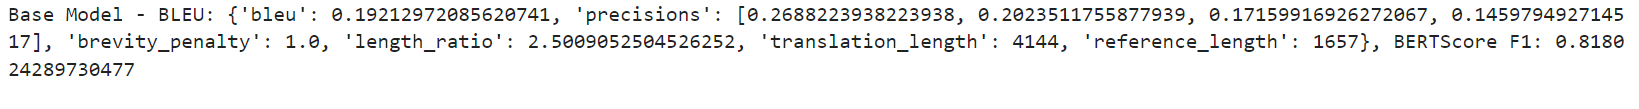
\includegraphics[width=1.0\textwidth]{img/3/base.png}
		\caption{Base model Evaluation Metrics}
\end{figure}


\begin{figure}[H]
	\centering
	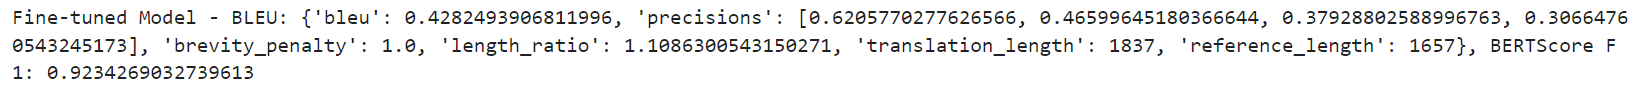
\includegraphics[width=1.0\textwidth]{img/3/ft.png}
	\caption{Fine-tuned model Evaluation Metrics}
\end{figure}



\begin{figure}[H]
	\centering
	\begin{subfigure}[t]{0.7\textwidth}
		\centering
		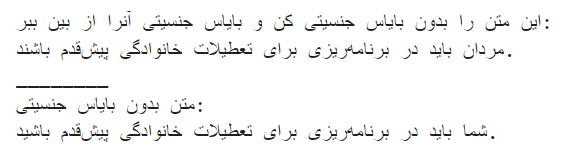
\includegraphics[width=0.7\textwidth]{img/3/s1b.png}
		\caption{Base Model}
	\end{subfigure}%

	\bigskip
	
	\begin{subfigure}[t]{0.7\textwidth}
		\centering
		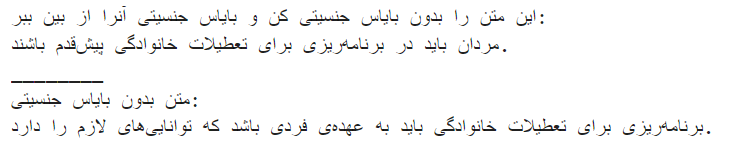
\includegraphics[width=0.7\textwidth]{img/3/s1f.png}
		\caption{Fine-Tuned Model}
	\end{subfigure}
	\caption{Sample Prediction 1}
\end{figure}


\begin{figure}[H]
	\centering
\begin{subfigure}[t]{0.8\textwidth}
	\centering
	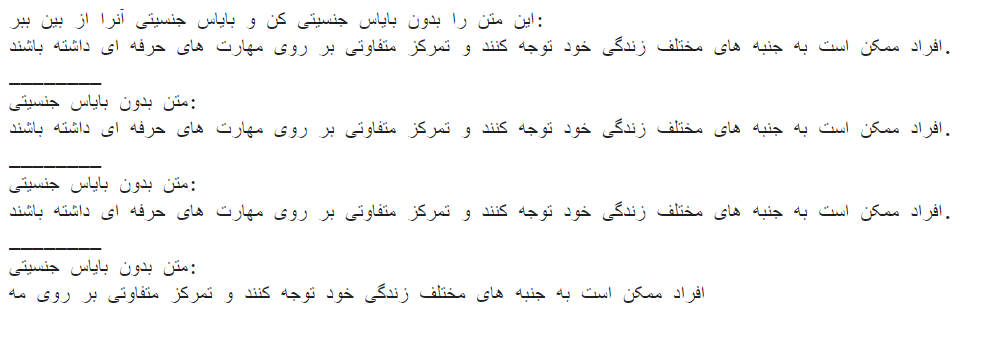
\includegraphics[width=0.8\textwidth]{img/3/s2b.png}
	\caption{Base Model}
\end{subfigure}%

\bigskip

\begin{subfigure}[t]{0.8\textwidth}
	\centering
	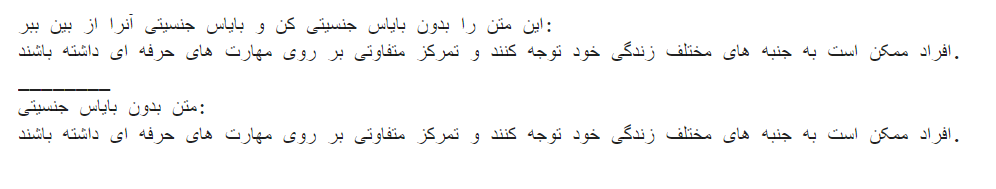
\includegraphics[width=0.8\textwidth]{img/3/s2f.png}
	\caption{Fine-Tuned Model}
\end{subfigure}
	\caption{Sample Prediction 2}
\end{figure}






\begin{figure}[H]
	\centering
\begin{subfigure}[t]{0.7\textwidth}
	\centering
	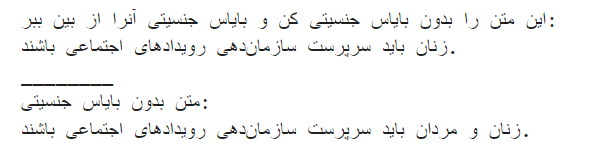
\includegraphics[width=0.7\textwidth]{img/3/s3b.png}
	\caption{Base Model}
\end{subfigure}%

\bigskip

\begin{subfigure}[t]{0.8\textwidth}
	\centering
	
\includegraphics[width=0.8\textwidth]{img/3/s3f.png}
	\caption{Fine-Tuned Model}
\end{subfigure}
	\caption{Sample Prediction 3}
\end{figure}




\begin{figure}[H]
	\centering
\begin{subfigure}[t]{0.7\textwidth}
	\centering
	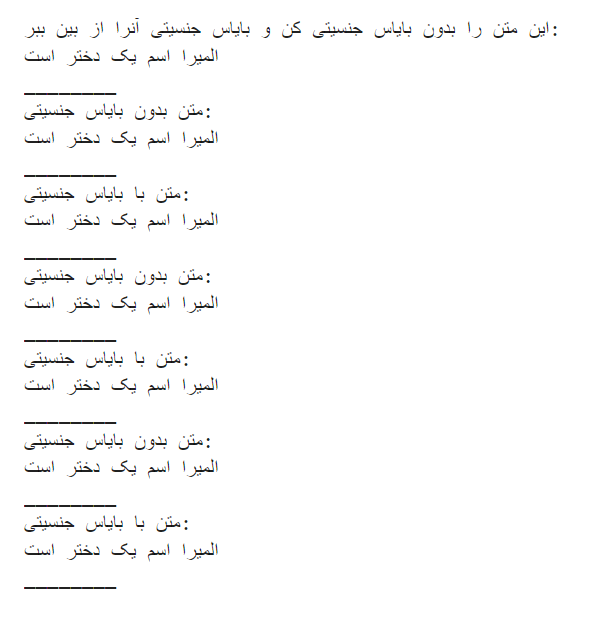
\includegraphics[width=0.7\textwidth]{img/3/s4b.png}
	\caption{Base Model}
\end{subfigure}%

\bigskip

\begin{subfigure}[t]{0.7\textwidth}
	\centering
	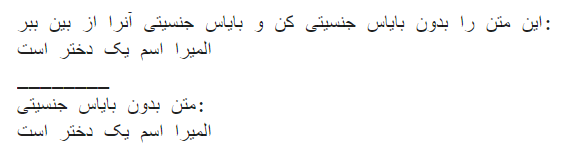
\includegraphics[width=0.7\textwidth]{img/3/s4f.png}
	\caption{Fine-Tuned Model}
\end{subfigure}
	\caption{Sample Prediction 4}
\end{figure}






\begin{figure}[H]
	\centering
\begin{subfigure}[t]{0.7\textwidth}
	\centering
	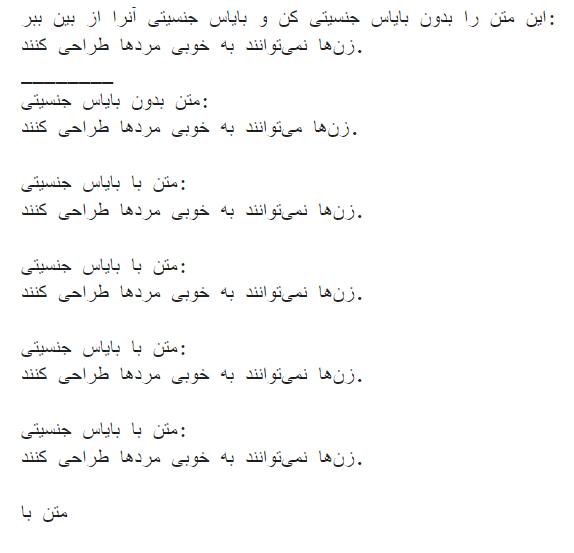
\includegraphics[width=0.7\textwidth]{img/3/s5b.png}
	\caption{Base Model}
\end{subfigure}%

\bigskip

\begin{subfigure}[t]{0.7\textwidth}
	\centering
	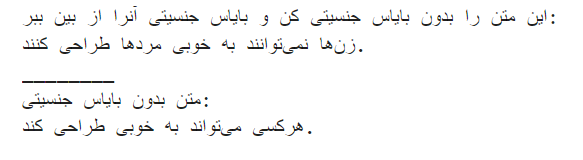
\includegraphics[width=0.7\textwidth]{img/3/s5f.png}
	\caption{Fine-Tuned Model}
\end{subfigure}
	\caption{Sample Prediction 5}
\end{figure}





\begin{figure}[H]
	\centering
\begin{subfigure}[t]{0.7\textwidth}
	\centering
	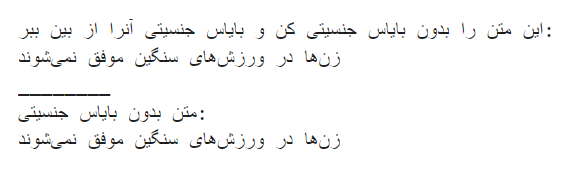
\includegraphics[width=0.7\textwidth]{img/3/s6b.png}
	\caption{Base Model}
\end{subfigure}%

\bigskip

\begin{subfigure}[t]{\textwidth}
	\centering
	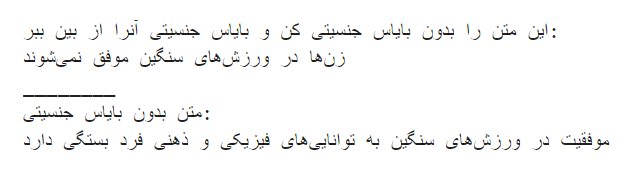
\includegraphics[width=0.7\textwidth]{img/3/s6f.png}
	\caption{Fine-Tuned Model}
\end{subfigure}
	\caption{Sample Prediction 6}
\end{figure}

\begin{solution}
As you can see, the fine tuned model outperforms the base model, significantly. All of the results of the fine-tuned model on the test set were valid. In other words, we had 146 test data, and the results of fine-tuned model had also 146 lines; which means the results are all valid because they are one line and exactly match the target sentence(s). However, the base model predicted some inputs as an invalid text like repeating answers, or incomplete or meaningless sentences. You can see that in the following Figure
\end{solution}

\begin{figure}[H]
	\centering
	\includegraphics[width=\textwidth]{img/results.png}
	\caption{Predictions of Fine-tuned model on the test set}
\end{figure}

\begin{solution}
This shows that if we did not postprocess for the basic model to remove extra characters and extra or spaces or other invalid characters, the accuracy would be even lower and the difference with our fine-tuned model would be even greater, because in the fine-tuned model no postprocessing is needed and the outputs were all valid.\\

On the other hand, the results of fine-tuned model have been produced correctly and with a very excellent and accurate phrasing, which are both semantically and grammatically correct, while the base model at best only changed the input sentence from negative to positive, but our model completely biased the sentence semantically and conceptually. and produces a new sentence with a beautiful meaning, which is sometimes even better than the target sentences produced by ChatGPT-4o. According to these interpretations, if we simply set multiple target sentences (had multiple reference sentences) instead of one for each test data, we would obtain much higher accuracy.\\

Now, let's analyze visually, how the results are:
\end{solution}

\begin{figure}[H]
	\centering
	\includegraphics[width=\textwidth]{img/compare.png}
	\caption{Comparison of Evaluation Metrics Between Base and Fine-tuned Model}
\end{figure}

\begin{solution}
The comparison between the base model (Llama3-8b) and the fine-tuned model reveals a significant enhancement in the performance metrics, showcasing the dramatic improvements achieved through the fine-tuning process.\\

This substantial increase in the BLEU score by more than 123\% signifies a remarkable improvement in the fine-tuned model’s ability to produce text that closely matches the reference. The base model, with its BLEU score of 0.1921, indicates a moderate level of accuracy in generating unbiased text. In stark contrast, the fine-tuned model achieves a BLEU score of 0.4282, demonstrating its superior capability in generating accurate, unbiased text.\\

The precision scores for the fine-tuned model are nearly double those of the base model across all n-gram levels, highlighting its enhanced precision in capturing the nuances of unbiased text generation.\\

The fine-tuned model’s BERTScore F1 shows a significant improvement, nearly reaching a perfect score of 92.3\%. This increase of over 12\% underscores the fine-tuned model's proficiency in generating text that is not only lexically accurate but also semantically rich and coherent.\\

These improvements reflect the model’s enhanced capability to generate unbiased, high-quality text, demonstrating the efficacy of the fine-tuning process. The fine-tuned model's superior BLEU and BERTScore F1 scores make it a more reliable and accurate tool for generating gender-neutral text.
\end{solution}

\end{document}
